%{{{1
\documentclass[ignorenonframetext,]{beamer}
\setbeamertemplate{caption}[numbered]
\setbeamertemplate{caption label separator}{: }
\setbeamercolor{caption name}{fg=normal text.fg}
\beamertemplatenavigationsymbolsempty
\usepackage{lmodern}
\usepackage{amssymb,amsmath}
\usepackage{ifxetex,ifluatex}
\usepackage{fixltx2e} % provides \textsubscript
\ifnum 0\ifxetex 1\fi\ifluatex 1\fi=0 % if pdftex
  \usepackage[T1]{fontenc}
  \usepackage[utf8]{inputenc}
\else % if luatex or xelatex
  \ifxetex
    \usepackage{mathspec}
  \else
    \usepackage{fontspec}
  \fi
  \defaultfontfeatures{Ligatures=TeX,Scale=MatchLowercase}
\fi
\usetheme{alui}
% use upquote if available, for straight quotes in verbatim environments
\IfFileExists{upquote.sty}{\usepackage{upquote}}{}
% use microtype if available
\IfFileExists{microtype.sty}{%
\usepackage{microtype}
\UseMicrotypeSet[protrusion]{basicmath} % disable protrusion for tt fonts
}{}
\newif\ifbibliography
\usepackage{natbib}
\bibliographystyle{plainnat}
\usepackage{color}
\usepackage{fancyvrb}
\newcommand{\VerbBar}{|}
\newcommand{\VERB}{\Verb[commandchars=\\\{\}]}
\DefineVerbatimEnvironment{Highlighting}{Verbatim}{commandchars=\\\{\}}
% Add ',fontsize=\small' for more characters per line
\newenvironment{Shaded}{}{}
\newcommand{\KeywordTok}[1]{\textcolor[rgb]{0.00,0.44,0.13}{\textbf{{#1}}}}
\newcommand{\DataTypeTok}[1]{\textcolor[rgb]{0.56,0.13,0.00}{{#1}}}
\newcommand{\DecValTok}[1]{\textcolor[rgb]{0.25,0.63,0.44}{{#1}}}
\newcommand{\BaseNTok}[1]{\textcolor[rgb]{0.25,0.63,0.44}{{#1}}}
\newcommand{\FloatTok}[1]{\textcolor[rgb]{0.25,0.63,0.44}{{#1}}}
\newcommand{\ConstantTok}[1]{\textcolor[rgb]{0.53,0.00,0.00}{{#1}}}
\newcommand{\CharTok}[1]{\textcolor[rgb]{0.25,0.44,0.63}{{#1}}}
\newcommand{\SpecialCharTok}[1]{\textcolor[rgb]{0.25,0.44,0.63}{{#1}}}
\newcommand{\StringTok}[1]{\textcolor[rgb]{0.25,0.44,0.63}{{#1}}}
\newcommand{\VerbatimStringTok}[1]{\textcolor[rgb]{0.25,0.44,0.63}{{#1}}}
\newcommand{\SpecialStringTok}[1]{\textcolor[rgb]{0.73,0.40,0.53}{{#1}}}
\newcommand{\ImportTok}[1]{{#1}}
\newcommand{\CommentTok}[1]{\textcolor[rgb]{0.38,0.63,0.69}{\textit{{#1}}}}
\newcommand{\DocumentationTok}[1]{\textcolor[rgb]{0.73,0.13,0.13}{\textit{{#1}}}}
\newcommand{\AnnotationTok}[1]{\textcolor[rgb]{0.38,0.63,0.69}{\textbf{\textit{{#1}}}}}
\newcommand{\CommentVarTok}[1]{\textcolor[rgb]{0.38,0.63,0.69}{\textbf{\textit{{#1}}}}}
\newcommand{\OtherTok}[1]{\textcolor[rgb]{0.00,0.44,0.13}{{#1}}}
\newcommand{\FunctionTok}[1]{\textcolor[rgb]{0.02,0.16,0.49}{{#1}}}
\newcommand{\VariableTok}[1]{\textcolor[rgb]{0.10,0.09,0.49}{{#1}}}
\newcommand{\ControlFlowTok}[1]{\textcolor[rgb]{0.00,0.44,0.13}{\textbf{{#1}}}}
\newcommand{\OperatorTok}[1]{\textcolor[rgb]{0.40,0.40,0.40}{{#1}}}
\newcommand{\BuiltInTok}[1]{{#1}}
\newcommand{\ExtensionTok}[1]{{#1}}
\newcommand{\PreprocessorTok}[1]{\textcolor[rgb]{0.74,0.48,0.00}{{#1}}}
\newcommand{\AttributeTok}[1]{\textcolor[rgb]{0.49,0.56,0.16}{{#1}}}
\newcommand{\RegionMarkerTok}[1]{{#1}}
\newcommand{\InformationTok}[1]{\textcolor[rgb]{0.38,0.63,0.69}{\textbf{\textit{{#1}}}}}
\newcommand{\WarningTok}[1]{\textcolor[rgb]{0.38,0.63,0.69}{\textbf{\textit{{#1}}}}}
\newcommand{\AlertTok}[1]{\textcolor[rgb]{1.00,0.00,0.00}{\textbf{{#1}}}}
\newcommand{\ErrorTok}[1]{\textcolor[rgb]{1.00,0.00,0.00}{\textbf{{#1}}}}
\newcommand{\NormalTok}[1]{{#1}}

% Prevent slide breaks in the middle of a paragraph:
\widowpenalties 1 10000
\raggedbottom

\AtBeginPart{
  \let\insertpartnumber\relax
  \let\partname\relax
  \frame{\partpage}
}
\AtBeginSection{
  \ifbibliography
  \else
    \let\insertsectionnumber\relax
    \let\sectionname\relax
    \frame{\sectionpage}
  \fi
}
\AtBeginSubsection{
  \let\insertsubsectionnumber\relax
  \let\subsectionname\relax
  \frame{\subsectionpage}
}

\setlength{\emergencystretch}{3em}  % prevent overfull lines
\providecommand{\tightlist}{%
  \setlength{\itemsep}{0pt}\setlength{\parskip}{0pt}}
\setcounter{secnumdepth}{0}
\usepackage[T1]{fontenc}
\usepackage{amssymb,bm,mathtools,amsmath,bbm}
\usepackage{graphicx,caption,float}
\def\beginmyfig{\begin{figure}[H]\begin{center}}
\def\endmyfig{\end{center}\end{figure}}
\newcommand{\tbf}[1]{\textbf{#1}}
\newcommand{\iid}{\overset{iid}{\sim}}
\def\inv{^{\raisebox{.2ex}{$\scriptscriptstyle-1$}}}
\newcommand{\m}[1]{\mathbf{\bm{#1}}}
\newcommand{\norm}[1]{\left\lVert#1\right\rVert}
\newcommand{\p}[1]{\left(#1\right)}
\newcommand{\bk}[1]{\left[#1\right]}
\newcommand{\bc}[1]{ \left\{#1\right\} }
\newcommand{\abs}[1]{ \left|#1\right| }
\newcommand{\mat}{ \begin{pmatrix} }
\newcommand{\tam}{ \end{pmatrix} }
\newcommand{\suml}{ \sum_{i=1}^n }
\newcommand{\prodl}{ \prod_{i=1}^n }
\newcommand{\ds}{ \displaystyle }
\newcommand{\df}[2]{ \frac{d#1}{d#2} }
\newcommand{\ddf}[2]{ \frac{d^2#1}{d{#2}^2} }
\newcommand{\pd}[2]{ \frac{\partial#1}{\partial#2} }
\newcommand{\pdd}[2]{\frac{\partial^2#1}{\partial{#2}^2} }
\newcommand{\N}{ \mathcal{N} }
\newcommand{\E}{ \text{E} }
\def\given{~\bigg|~}
\title[Bayesian FAM for CyTOF Data]{Bayesian Feature Allocation Models for Natural Killer Cell Repertoire Studies Using Mass Cytometry Data}
\author[A. Lui]{Arthur Lui \\ {\small Advisor$\colon$ Juhee Lee}}
\institute{Department of Applied Mathematics and Statistics\\ UC Santa Cruz}
\def\logit{\text{logit}}
\newcommand{\true}{{\mbox{\tiny TR}}}
\newcommand{\bZ}{\mbox{\boldmath $Z$}}
\newcommand{\bp}{\mbox{\boldmath $p$}}
\newcommand{\bq}{\mbox{\boldmath $q$}}
\newcommand{\bz}{\mbox{\boldmath $z$}}
\newcommand{\bw}{\mbox{\boldmath $w$}}
\newcommand{\bW}{\mbox{\boldmath $W$}}
\newcommand{\bI}{\mbox{\boldmath $I$}}
\newcommand{\ind}{\overset{ind}{\sim}}
\newcommand{\Ind}[1]{\mathbbm{1}\bc{#1}}
\newcommand{\by}{\mbox{\boldmath $y$}}
\def\bmu{\bm{\mu}}
\def\bnu{\bm{\nu}}
\def\bomega{\bm{\omega}}
\def\bgam{\bm{\gamma}}
\def\bsig{\bm{\sigma}}
\def\blambda{\bm{\lambda}}
\def\bet{\bm{\eta}}
\def\lin{\lambda_{in}}
\def\h{\bm{h}}
\def\mus{\mu^\star}
\def\sss{{\sigma^2}^\star}
\usepackage{appendixnumberbeamer}
\def\eye{\bm{\mathrm{I}}}
%}}}1
\begin{document}

\begin{frame}
\date{8 June 2018}
\titlepage
\end{frame}

\begin{frame}{Introduction}
\begin{itemize}
\item
  \textbf{Cytometry at time-of-flight (CyTOF)} \setlength\itemsep{1em}
  \begin{minipage}{\textwidth}
  \begin{columns}[T]
  \begin{column}{0.1\textwidth}
  \vspace{5em}
  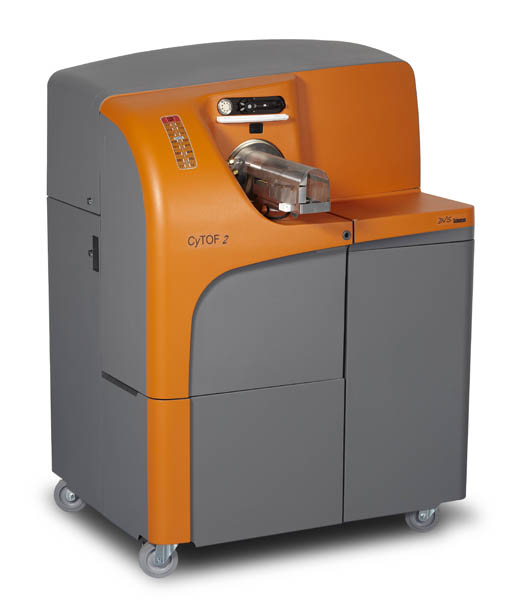
\includegraphics[scale=0.5]{img/CyTOF_instrument.jpg}
  \end{column}
  \begin{column}{0.6\textwidth}
  \begin{itemize}
  \item
  commercialized in 2009
  \item 
  makes use of time-of-flight mass spectrometry to accelerate, separate, and
  identify ions by mass
  \item
  enables detection of many parameters (biological, phenotypic, or functional
  markers) in less time and at a higher resolution \citep{cheung2011screening}
  \item 
  led to greater understanding of natural killer (NK) cells
  \end{itemize}
  \end{column}
  \end{columns}
  \end{minipage}
\end{itemize}
\end{frame}

\begin{frame}{Introduction}
  \begin{itemize}
    \setlength\itemsep{1em}
    \item
      \textbf{Natural Killer cells} play a critical role in cancer immunosurveillance
    \item NK cell diversity refers to number of NK cell sub-populations within
      NK cells, and also affects antiviral response
    \item Drs. Thall and Rezvani, collaborators at UT MD Anderson Cancer
      Center, have conducted clinical trials to study the potential clinical
      efficacy of umbilical cord blood (UCB) transplantation as a therapy for
      leukemia.
    \item In the trials, leukemia patients received UCB cell transplants, and
      NK cell surface protein markers are measured using mass cytometry.
    \item UCB NK cell therapy has the advantage of low risk of viral
      transmission from donor to recipient \citep{sarvaria2017umbilical}.
  \end{itemize}
\end{frame}

\begin{frame}{CyTOF Data}

\begin{table}
\begin{tabular}{r|rrrrrrr}
  \hline
  & 2B4 & 2DL1 & 2DL3 & 2DS4 & 3DL1 & CCR7 & $\cdots$ \\
  \hline
  1 & 47.60 & 0.00 & 30.90 & 1.35 & 82.49 & 0.00 & $\cdots$ \\
  2 & 81.84 & 0.44 & 0.88 & 0.51 & 176.99 & 2.38 & $\cdots$ \\
  3 & 13.33 & 0.00 & 0.00 & 0.00 & 0.00 & 8.81   & $\cdots$ \\
  4 & 23.64 & 3.37 & 43.39 & 0.27 & 0.73 & 0.00  & $\cdots$ \\
  5 & 156.19 & 0.00 & 9.04 & 0.00 & 0.00 & 11.43 & $\cdots$ \\
  6 & 273.86 & 0.00 & 9.71 & 2.41 & 0.84 & 0.52  & $\cdots$ \\
  $\vdots$ & $\vdots$& $\vdots$& $\vdots$& $\vdots$& $\vdots$& $\vdots$& \\
  \hline
  Cutoff & 7.62 & 6.07 & 13.60 & 3.79 & 15.50 & 9.52 & $\cdots$\\
  \hline
\end{tabular}
\caption{Cord-blood sample marker expression levels for 6 of 32 NK-cell markers
(columns), and 6 of 41474 cells (rows). Last row contains cutoff values
returned by CyTOF instrument.}
\end{table}

\begin{itemize}
\tightlist
\item
  Data missing not at random

  \begin{itemize}
  \tightlist
  \item
    Some markers contain up to 85\% missing values
  \end{itemize}
\item
  Cutoff values are computed after measurement
\end{itemize}

\end{frame}

\begin{frame}{CyTOF Data}

\begin{table}
\begin{tabular}{r|rrrrrrr}
  \hline
  & 2B4 & 2DL1 & 2DL3 & 2DS4 & 3DL1 & CCR7 & $\cdots$ \\
  \hline
  1 & 1 & 0 & 1 & 0 & 1 & 0 & $\cdots$ \\
  2 & 1 & 0 & 0 & 0 & 1 & 0 & $\cdots$ \\
  3 & 1 & 0 & 0 & 0 & 0 & 0 & $\cdots$ \\
  4 & 1 & 0 & 1 & 0 & 0 & 0 & $\cdots$ \\
  5 & 1 & 0 & 0 & 0 & 0 & 1 & $\cdots$ \\
  6 & 1 & 0 & 0 & 0 & 0 & 0  & $\cdots$ \\
  $\vdots$ & $\vdots$& $\vdots$& $\vdots$& $\vdots$& $\vdots$& $\vdots$& \\
  \hline
  Cutoff & 7.62 & 6.07 & 13.60 & 3.79 & 15.50 & 9.52 & $\cdots$\\
  \hline
\end{tabular}
\caption{Cell phenotypes (rows)}
\end{table}

\begin{itemize}
\tightlist
\item
  Obtaining cell phenotypes using overly-simplistic methods may yield
  unreasonably high number of sub-populations.
\end{itemize}

\end{frame}

\begin{frame}{Existing Methods}

\begin{itemize}
\setlength\itemsep{1em}
  \item Most existing methods use traditional clustering methods (K-means,
    hierarchical clustering, density-based clustering, nearest-neighbor
    clustering, etc.)
  \item For high-dimensional cytometry data, \cite{weber2016comparison}
    compared existing clustering methods including \textbf{FlowSOM}
    \citep{van2015flowsom}, \textbf{PhenoGraph} \citep{levine2015data}, 
    \textbf{Rclusterpp} \citep{linderman2013package}, 
    and \textbf{flowClust} \citep{lo2009flowclust}
  \item
    Existing methods do not directly model latent phenotypes or quantify model
    uncertainty
  \end{itemize}
\end{frame}

\begin{frame}{Proposed Projects}

\begin{itemize}
\tightlist
\item
  \textbf{Project I}: Bayesian Feature Allocation Model for
  Heterogeneous Cell Populations \setlength\itemsep{1em}
\item
  \textbf{Project II}: Repulsive Feature Allocation Model
\item
  \textbf{Project III}: Feature Allocation Model with Regression for
  Abundances of Features in Longitudinal Data
\end{itemize}
\end{frame}

% Project I %%%%%%%%%%%%%%%%%%%%%%%%%%%%%%%%%%%%%%%%%%%
\frame[noframenumbering, plain]{
  \begin{center} \Huge \textbf{Project I} \end{center} 
}

\frame{ %
  \frametitle{Feature Allocation Model -- Indian buffet process}
  \vspace{5mm}

  \cite{griffiths2011indian} introduced the
  IBP as follows:
  \vspace{5mm}

  Let $\bm Z$ be a $J\times K$ matrix such that
  $$
  \begin{array}{rclcl}
    z_{jk} &\mid& \pi_k  &\sim& \text{Bernoulli}(\pi_k) \\
    \pi_k  &\mid& \alpha &\sim& \text{Beta}\p{\frac{\alpha}{K},1} \\ 
  \end{array}
  $$
  for $j=1,\cdots J$ and $k=1,\cdots, K$, and where $\alpha$ is positive. \\
  \pause

  Then as $K\rightarrow \infty$, $\bm Z \sim \text{IBP}(\alpha)$.
  It can be shown that
  $$
  \text{P}(\bm Z) = \frac{\alpha^{K_+}}{\prod_{h=1}^{2^J-1} 
                          {K_h}!} 
                          \exp\{-\alpha H_J\}\prod_{k=1}^{K_+}
                                       \frac{(J-m_k)!(m_k-1)!}{J!},
  $$

  where $H_J=\sum_{j=1}^J j^{-1}$ is the harmonic number, $K_+$ is
  the number of non-zero columns in $\bm Z$, $m_k$ is the $k^{th}$
  column sum of $\bm Z$, and $K_h$ the number of columns having
  history $h$ (some binary number).
}


% Draws from IBP
\frame{ %
  \frametitle{One draw from the IBP}
  \vspace{5mm}
  \beginmyfig
    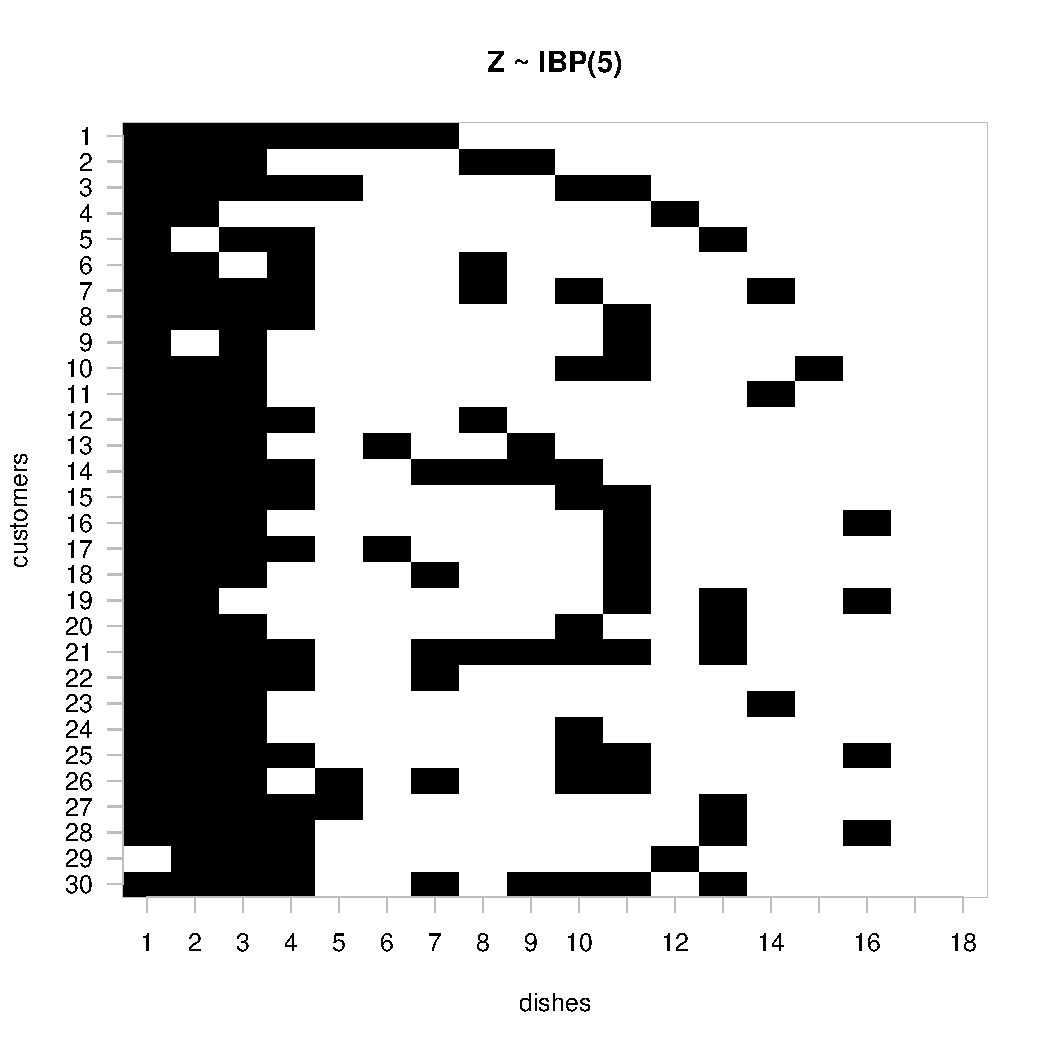
\includegraphics[scale=.4]{img/ibp/Z.pdf}
    %\caption{Put Caption Here}
  \endmyfig
}


\begin{frame}{Project I: Bayesian Feature Allocation Model for
Heterogeneous Cell Populations}

\begin{block}{Notation}

\begin{itemize}
\tightlist
\item
  \(I\): Number of samples
\item
  \(J\): Number of markers
\item
  \(N_i\): Number of observations in sample \(i\)
\item
  \(\tilde{y}_{inj}\): Raw expression levels for observation \(n\) in
  sample \(i\) for marker \(j\). \((\tilde y_{inj} \ge 0)\)
\item
  \(c_{ij}\): Cutoff for marker \(j\), sample \(i\)
\item
  \(y_{inj}\): Transformed expression levels for observation \(n\),
  sample \(i\), marker \(j\) \[
  y_{inj}=\log\p{\frac{\tilde{y}_{inj}}{c_{ij}}} \in \mathbb{R}.
  \]

  \begin{itemize}
  \tightlist
  \item
    \((y_{inj} \gg 0)\) likely corresponds to expression
  \item
    \((y_{inj} \ll 0)\) likely corresponds to non-expression
  \end{itemize}
\end{itemize}

\end{block}

\end{frame}

\begin{frame}{Project I: Bayesian Feature Allocation Model for
Heterogeneous Cell Populations}

\begin{itemize}
%\tightlist
\item $K$ is a sufficiently large constant
\item
  \(\bZ\): \((J \times K)\) binary matrix defining the latent
  phenotypes.

  \begin{itemize}
  \item
    if \(Z_{jk} = 1\), then marker \(j\) is expressed in phenotype \(k\)
  \item
    if \(Z_{jk} = 0\), then marker \(j\) is not expressed in phenotype
    \(k\)
  \end{itemize}
\item
  \(\lambda_{in} \in \bc{1,...,K}\): The latent phenotype of observation
  \(n\), sample \(i\)
\end{itemize}
\end{frame}

\begin{frame}{Project I: Sampling Distribution}
\begin{align*}
y_{inj} \mid \bet_{ij}, \bmu^\star, \bsig^{2 \star}_{i} \ind
\begin{cases}
   F_0, &\mbox{if $z_{j,\lambda_{in}}=0$},\\
   F_1, &\mbox{if $z_{j,\lambda_{in}}=1$}.\\
\end{cases} \label{eq:y-mix}
\end{align*}
%
\begin{itemize}
\item $F_0 = \sum_{\ell=1}^{L^0} \eta^0_{ij\ell}~\text{Normal}(\mu^\star_{0\ell}, \sigma^{2 \star}_{0i\ell})$, where $\mu^\star_{0\ell} < 0$
\item $F_1 = \sum_{\ell=1}^{L^1} \eta^1_{ij\ell}~\text{Normal}(\mu^\star_{1\ell}, \sigma^{2 \star}_{1i\ell})$, where $\mu^\star_{1\ell} > 0$
%\item
%  Fixed number of mixture components \(L^0\) and \(L^1\)
%\item
%  Mixture weights \(\bet^0_{ij}\) and \(\bet^1_{ij}\) where
%  \(\sum_{\ell=1}^{L^0} \eta^0_{ij\ell}=\sum_{\ell=1}^{L^1}\eta^1_{ij\ell}=1\),
%  and \(\eta^0_{ij\ell}, \eta^1_{ij\ell} > 0\)
\end{itemize}
%
\begin{figure}
  \begin{center}
    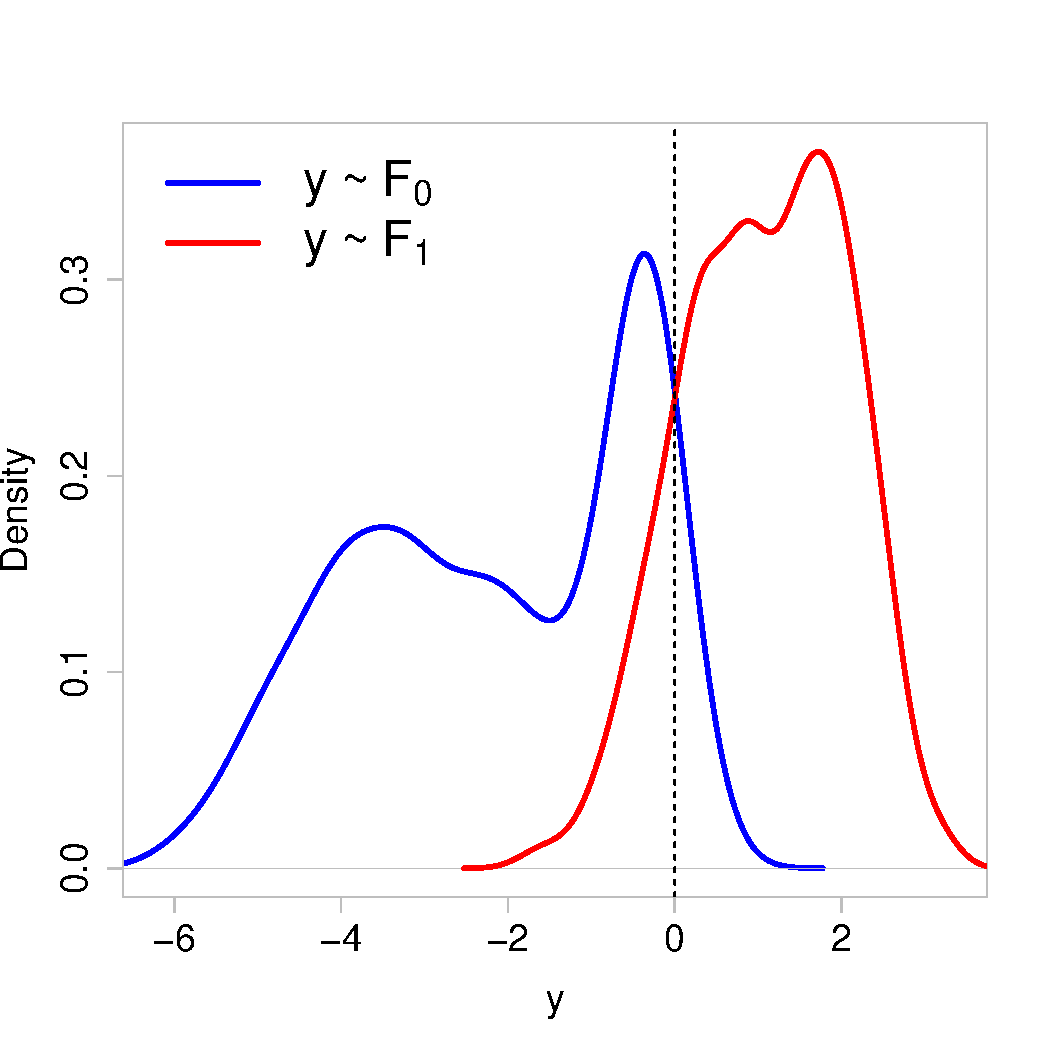
\includegraphics[scale=.2]{img/mixture.pdf}
    \caption{Kernel density estimate of samples from $F_0$ (blue) and $F_1$ (red)}
  \end{center}
\end{figure}
\end{frame}

\begin{frame}{Project I: Missing Mechanism}

$$
  m_{inj} \mid p_{inj} \ind \text{Bernoulli}(p_{inj})
$$
\pause
$$
  \logit(p_{inj}) = \begin{cases}
  \beta_{0i} - \beta_{1i}(y_{inj}-c_0)^2, & \text{if } y_{inj} < c_0\nonumber \\
  \beta_{0i} - \beta_{1i}c_1\p{y_{inj}-c_0}^{1/2}, & \text{otherwise}, \nonumber \\
  \end{cases} 
$$

where \(m_{inj}=1\) if \(y_{inj}\) is missing, and 0 otherwise.
\beginmyfig
\includegraphics[scale=.20]{../sampling/img/prob_miss_example.pdf}
\caption{Example missing mechanism} \endmyfig
\end{frame}

\begin{frame}{Project I: Priors}
\begin{block}{Latent Phenotypes}
\begin{eqnarray*}
  \bZ \mid \alpha &\sim& \text{IBP}_K(\alpha) \\
  \alpha &\sim& \text{Gamma}(a_\alpha, b_\alpha) \\
\end{eqnarray*}
\end{block}
\end{frame}

\begin{frame}[noframenumbering]{Project I: Priors}
\begin{block}{Latent Phenotypes}
\begin{eqnarray*}
  z_{jk} \mid v_k  &\ind& \text{Bernoulli}(v_k) \\
  v_k  \mid \alpha &\iid& \text{Beta}\p{\alpha/K,1} \\ 
  \alpha &\sim& \text{Gamma}(a_\alpha, b_\alpha) \\
\end{eqnarray*}
\end{block}
\end{frame}


\begin{frame}[noframenumbering]{Project I: Priors}
\begin{block}{Latent Phenotypes}
\begin{eqnarray*}
  z_{jk} \mid h_{jk}, v_k &=& 
  \mathbb{I}\bc{ \Phi(h_{jk} \mid 0, \alt<2>{\Gamma_{jj}}{1}) < v_k } \\
  v_k \mid \alpha &\iid& \text{Beta}(\alpha/K, 1) \\
  \h_k &\iid& \text{Normal}_J(\mathbf{0}, \alt<2>{\Gamma}{\eye}) \\ 
  \alpha &\sim& \text{Gamma}(a_\alpha, b_\alpha) \\
\end{eqnarray*}
\end{block}
\pause
\begin{itemize}
  \item Dependent IBP (dIBP) \citep{williamson2010dependent} construction to model correlations between markers
  \item dIBP reduces to IBP \citep{griffiths2011indian} when $\Gamma$ is the identity matrix
\end{itemize}
\end{frame}


\begin{frame}[noframenumbering]{Project I: Priors}
\begin{block}{Latent Phenotypes}
\begin{eqnarray*}
  \bZ \mid \alpha, \Gamma &\sim& \text{dIBP}_K(\alpha, \Gamma) \\
  \alpha &\sim& \text{Gamma}(a_\alpha, b_\alpha) \\
\end{eqnarray*}
\end{block}
\begin{itemize}
  \item Dependent IBP (dIBP) \citep{williamson2010dependent} construction to model correlations between markers
  \item dIBP reduces to IBP \citep{griffiths2011indian} when $\Gamma$ is the identity matrix
\end{itemize}
\end{frame}


\begin{frame}{Project I: Priors}
\begin{block}{Phenotype Abundance}
Let \(w_{ik}\) denote an abundance level of phenotype \(k\) in sample
\(i\). Let \(\bw_i=(w_{i1}, \ldots, w_{iK})\). Then,
\(\bw_{i} \mid K \iid \text{Dirichlet}_K(d/K)\).
\end{block}

\begin{block}{Latent Cell Phenotype Indicators}
\[p(\lin=k \mid \bm \bw_i) = w_{ik}\]
\end{block}
\end{frame}

\begin{frame}{Project I: Priors}
\begin{align*}
\mus_{0\ell} \mid \psi_0, \tau^2_0 &\iid \text{Normal}_-(\psi_0, \tau^2_0), ~~~ \ell \in \bc{1,...,L^0} \\
\mus_{1\ell} \mid \psi_1, \tau^2_1 &\iid \text{Normal}_+(\psi_1, \tau^2_1), ~~~ \ell \in \bc{1,...,L^1} \\
\sigma^2_{0i\ell} \mid s_i &\ind \text{Inverse-Gamma}(a_\sigma, s_i), ~~~ \ell \in \bc{1,...,L^0} \\
\sigma^2_{1i\ell} \mid s_i &\ind \text{Inverse-Gamma}(a_\sigma, s_i), ~~~ \ell \in \bc{1,...,L^1}  \\
  s_i &\iid \text{Gamma}(a_s, b_s), ~~~ i \in \bc{1,...,I} \\
\bm\eta^0_{ij} &\iid \text{Dirichlet}_{L^0}(a_{\eta^0}/L^0), ~~~ i \in \bc{1,...,I}, j \in \bc{1,...,J} \\
\bm\eta^1_{ij} &\iid \text{Dirichlet}_{L^1}(a_{\eta^1}/L^1), ~~~ i \in \bc{1,...,I}, j \in \bc{1,...,J} \\
\beta_{0i} &\iid \text{Normal}(m_{\beta_0}, s^2_{\beta_0}), ~~~ i \in \bc{1,...,I} \\
\beta_{1i} &\iid \text{Normal}_+(m_{\beta_1}, s^2_{\beta_1}), ~~~ i \in \bc{1,...,I} \\
\end{align*}
\end{frame}

\begin{frame}{Project I: Posterior Estimate for $\bZ$}
  \begin{itemize}
    \setlength\itemsep{1em}
    \item $\bZ$ susceptible to label switching, especially when $K$ is random
    \item We summarize the posterior distribution of $\bZ$ using sequentially-allocated latent structure optimization (SALSO) \citep{salso}
  \end{itemize}
\end{frame}

\begin{frame}{Project I: Posterior Estimate for $\bZ$}
For each posterior sample $b\in \bc{1,...,B}$ and patient sample $i$,
\begin{enumerate}
\item compute a $(J\times J)$ Adjacency Matrix $A_i^{(b)}$, where
  $$
  A^{(b)}_{i_{j,j'}} = \sum_{k=1}^K w^{(b)}_{ik} 
  \Ind{ z^{(b)}_{jk} = z^{(b)}_{j^\prime k} = 1}
  $$
\item compute the mean adjacency matrix \(\bar A_i = \sum_{b=1}^B A_i^{(b)} /
B\).
\item $\hat{\bm Z}_i = \text{argmin}_{\bm Z} \sum_{j,j'} (A_{i_{j,j'}}^{(b)} - \bar A_{i_{j,j'}})^2$
\end{enumerate}
\end{frame}

\begin{frame}{Project I: Simulation Study}
\begin{figure}
\begin{center}
\begin{tabular}{c}
\includegraphics[scale=.30]{../sampling/img/sim/Z1_true_noTranspose.pdf}
\end{tabular}
\end{center}
\vspace{-0.05in} \caption{Simulation truth for $\bZ$ in Sample 1, with markers in
rows and latent phenotypes in columns. Black and white represents
$z_{jk}=1$ and 0, respectively. The phenotypes and $\bw_1$ are
shown at the bottom and on top, respectively. The markers
are sorted by $w_{ik}$.}
%\vspace{-0.05in} \caption{Simulation truth for $\bZ$ in Sample 1, with markers in
%rows and latent phenotypes in columns. Black and white represents
%$z^\true_{jk}=1$ and 0, respectively. The phenotypes and $\bw^\true_1$ are
%shown on the left and right sides of each panel, respectively. The samples
%share the same $\bZ^\true$ and the phenotypes are arranged in order of
%$w_{ik}^\true$ within each sample.}
\end{figure}
\end{frame}

\begin{frame}{Project I: Simulation Study}
\begin{figure}
\begin{center}
\begin{tabular}{c}
\includegraphics[scale=.35]{../sampling/img/sim/Y001.png}
\end{tabular}
\end{center}
\vspace{-0.05in} \caption{Simulated data for one sample}
\end{figure}
\end{frame}

\begin{frame}{Project I: Simulation Results -- FAM}
\vspace{-1em}\begin{figure}
  \begin{center}
  \begin{tabular}{cc}
  \includegraphics[scale=.3]{../sampling/img/sim/YZ001.png}&
  \includegraphics[scale=.3]{../sampling/img/sim/Z1_true.pdf}\\
  {\small (a) Sample 1} & {\small(b) Z true} \\
  \end{tabular}
  \end{center}
  \vspace{-0.05in}
  \caption{FAM Simulation Study}
\end{figure}
\end{frame}

\begin{frame}[noframenumbering]{Missing Mechanism Posterior}
\vspace{-1em}\begin{figure}
  \begin{center}
    \includegraphics[scale=.4]{../sampling/img/sim/miss_mech_posterior.pdf}
  \end{center}
  \vspace{-0.05in}
  \caption{Posterior missing mechanism for simulation study in Project I for sample 1 (red), 2 (green), and 3 (blue). Prior missing mechanism in grey.}
\end{figure}
\end{frame}

\begin{frame}{Project I: Simulation Results -- FlowSOM}
\vspace{-1em}\begin{figure}
  \begin{center}
  \begin{tabular}{cc}
  \includegraphics[scale=.3]{../sampling/img/FlowSOM/YZ001_FlowSOM_SIM.png}&
  \includegraphics[scale=.3]{../sampling/img/sim/Z1_true.pdf}\\
  {\small (a) Sample 1} & {\small(b) Z true} \\
  \end{tabular}
  \end{center}
  \vspace{-0.05in}
  \caption{FlowSOM Simulation Study}
\end{figure}
\end{frame}


\begin{frame}{Project I: Simulation Study -- Comparing FAM and FlowSOM}
We use the F-score to summarize the accuracy of the computed cluster labels.
The F-score is defined as the harmonic mean of precision and recall.

$$
F_1 = \frac{2}{\text{precision}^{-1} + \text{recall}^{-1}},
$$

\begin{itemize}
  \item precision $=\p{\text{true positives}}/\p{\text{true positives} + \text{false positives}}$ 
  \item recall $=\p{\text{true positives}} / \p{\text{true positives} + \text{false negatives}}$
  \item $F_1 \in \bk{0,1}$ with $F_1=1$ being a perfect score
\end{itemize}

% latex table generated in R 3.4.4 by xtable 1.8-2 package
% Wed Jun  6 01:06:34 2018
\begin{table}
\begin{center}
\begin{tabular}{rrr}
  \hline
 & F-score & Elapsed time (seconds) \\ 
  \hline
  FlowSOM & 0.490 & 6 \\ 
  FAM & 0.999 & 17472 \\ 
   \hline
\end{tabular}
\end{center}
\caption{F-score and elapsed time for simulated data for FAM and FlowSOM}
\end{table}
\end{frame}

\begin{frame}{Project I: Conclusions for Comparing FAM and FlowSOM}
  \begin{itemize}
    \setlength\itemsep{1em}
    \item FAM produces posterior distribution and estimates of latent phenotypes and their weights
    \item Choose $K$ sufficiently large
    \item Graph first two principal components to visually estimate $K$
    \item FlowSOM quickly produces point estimates of clusters
    \item In FlowSOM, additional ad-hoc criteria are needed to produce estimates of latent phenotypes and their abundance
    \item In FlowSOM, missing values need to be pre-imputed
  \end{itemize}
\end{frame}


\begin{frame}{Project I: Cord Blood Samples Data}
  \begin{itemize}
    \setlength\itemsep{1em}
    \item Three cord blood (CB) samples from MD Anderson Cancer Center
    \item Number of cells in each sample $N = (41474,10454,5177)$
    \item Number of markers $J=32$
    \item $K$ = 20
    \item MCMC: 2000 iterations, 1000 burn-in
  \end{itemize}
\end{frame}

\begin{frame}{Project I: CB Study}
\vspace{-1em}\begin{figure}
  \begin{center}
  \begin{tabular}{cc}
  \includegraphics[scale=.3]{../sampling/img/cb/YZ001.png} &
  \includegraphics[scale=.3]{../sampling/img/FlowSOM/YZ001_FlowSOM_CB.png} \\
  {\small Sample 1 (FAM)} & {\small Sample 1 (FlowSOM)} \\
  \end{tabular}
  \end{center}
  \vspace{-0.05in}
  \caption{CB data Sample 1, analyzed using FAM (left) and FlowSOM (right)}
\end{figure}
\end{frame}

\begin{frame}{Project I: Posterior Predictive for Observed Data}
\vspace{-1em}\begin{figure}
  \begin{center}
  \begin{tabular}{cc}
  \includegraphics[scale=.3]{../sampling/img/cb/pp_obs_i1_j1.pdf}&
  \includegraphics[scale=.3]{../sampling/img/cb/pp_obs_i1_j2.pdf}\\
  {\small (a) Sample 1, marker 1} & {\small (b) Sample 1, marker 2} \\
  \end{tabular}
  \end{center}
  \vspace{-0.05in}
  \caption{Observed data density for $y_{ij}$ in grey. Posterior predictive density for observed data in blue.}
\end{figure}
\end{frame}

\begin{frame}{Project I: Probability of Non-expression for Imputed Values}
\begin{figure}
\begin{center}
  \includegraphics[scale=0.30]{../sampling/img/cb/pz0_missy.pdf}
  \caption{Histogram of posterior probabilities $\hat{q}_{ij}$ of
  non-expression for missing for all $(i,j)$.  The peak at 1 suggests 
  a marker is not likely expressed if its expression level is
  missing.}
\end{center}
\end{figure}
\end{frame}


\begin{frame}[fragile]{R Package}
\begin{Shaded}
\begin{Highlighting}[]
\CommentTok{# R code for installing cytof3}

\KeywordTok{library}\NormalTok{(devtools)}
\NormalTok{repo =}\StringTok{ 'luiarthur/ucsc_litreview'}
\NormalTok{subdir =}\StringTok{ 'cytof/src/model3/cytof3'}
\KeywordTok{install_github}\NormalTok{(repo, }\DataTypeTok{subdir=}\NormalTok{subdir)}
\end{Highlighting}
\end{Shaded}
\end{frame}

% Project II %%%%%%%%%%%%%%%%%%%%%%%%%%%%%%%%%%%%%%%%%%%
\frame[noframenumbering, plain]{
  \begin{center} \Huge \textbf{Project II} \end{center} 
}



\begin{frame}{Project II: Repulsive Feature Allocation Model}
  \begin{itemize}
    \setlength\itemsep{1em}
    \item Similar or duplicated features may occur in feature allocation matrix under IBP prior
    \item Repulsion penalizes similar features in the prior, resulting in a parsimonious model
    \item Different approaches for repulsive models have been developed mostly
    in the context of mixture models \citep{petralia2012repulsive,
    quinlan2017parsimonious, xie2017bayesian, quinlan2017density}. 
  \end{itemize}
\end{frame}

\begin{frame}{Project II: Repulsive Feature Allocation Model}
  \begin{block}{Objective}
  \begin{itemize}
    \setlength\itemsep{1em}
    \item Develop a repulsive feature allocation model for parsimonious feature
      matrix
    %\item Extend previous model to include a sample-specific covariate and
    %  perform feature selection for groups of samples 
    \item Compare phenotypes present in healthy subject samples and cord blood samples
  \end{itemize}
\end{block}
\end{frame}

\begin{frame}{Project II: Feature Selection for Different Samples}
  \begin{itemize}
    \item Sample covariate $x_i$. Cord blood samples ($x_i=0$). Healthy subject samples ($x_i=1$).
    \begin{figure}
      \begin{tabular}{cccc}
      {CB} & {CB} & {subject} & {subject} \\
      \includegraphics[scale=.1]{../sampling/img/cb/YZ001.png} &
      \includegraphics[scale=.1]{../sampling/img/cb/YZ002.png} &
      \includegraphics[scale=.1]{../sampling/img/sim/YZ001.png} &
      \includegraphics[scale=.1]{../sampling/img/sim/YZ002.png} \\
      {$x_1=0$} & {$x_2=0$} & {$x_3=1$} & {$x_4=1$} \\
      \end{tabular}
    \end{figure}
    \pause
    \item Learn binary indicator $\delta_{xk}\in \{0, 1\}$, $x=0,1$, and
      $k=1,\ldots, K$, to indicate whether samples from $x$ possess phenotype
      $k$ 
    %\item $\delta_{xk} \mid p_x \ind \text{Bernoulli}(p_{x})$ and $p_x \iid
    %  \text{Beta}(a_p, b_p)$.
    %  \pause
    %\item Unnormalized cell phenotype abundances $\tilde w_{ik} \ind
    %  \text{Gamma}(a_W/K, 1)$, $i=1, \ldots, I$, and $k=1, \ldots, K$. 
    %  \pause
    %\item Relative abundances in sample $i$ from $x_i$ as $ w_{ik} =\tilde
    %  w_{ik} \delta_{x_i k}/\sum_{\ell=1}^K\tilde w_{i\ell} \delta_{x_i \ell}$.
    %\item Relative abundance $w_{ik}$ is exactly zero for $\delta_{x_ik}=0$. 
    %  \pause
    %\item Samples from $x$ have the same subset of phenotypes but can have
    %  different relative abundances over the selected phenotypes. 
    %  \pause
    %\item Phenotypes with $\delta_{0k}=\delta_{1k}=1$ appear in all samples,
    %  while some are present in only one type of samples. 
    %  \pause
    %\item The probability models for the other parameters remain unchanged as
    %  in Project 1.  
  \end{itemize}
  %Feature-selection by $\delta_{xk}$ efficiently
  %facilitates joint analysis of samples obtained from different sources. The
  %model also allows phenotypes to absent in all samples, implying that some
  %phenotypes are not used to describe any cells, providing a more parsimonious
  %representation of cell-populations in samples.
\end{frame}


\begin{frame}{Project II: rep-FAM Prior}
\begin{align*}
  \only<1>{
    P(\bZ \mid v) &\propto \prod_{k=1}^K  \bc{\prod_{j=1}^J
    v_k^{z_{jk}}(1-v_k)^{1-z_{jk}}} \\
  } \only<2> {
    P(\bZ \mid v, C_\phi) &\propto \prod_{k=1}^K  \bc{\prod_{j=1}^J
    v_k^{z_{jk}}(1-v_k)^{1-z_{jk}}} \times \\
    &\hspace{1em}\prod_{k_1=1}^{K-1}\prod_{k_2=k_1+1}^{K} \bc{1 -
    C_\phi\p{\rho(\bz_{k_1}, \bz_{k_2})}}\\
  }
  v_K \mid \alpha &\sim \text{Beta}(\alpha/K, 1)
\end{align*}
%
\pause
%
where
\begin{itemize}
  \setlength\itemsep{1em}
  \item $C_\phi(\cdot)$ is a continuous decreasing function in distance with
    $C_\phi(0)=1$ and $\lim_{d\rightarrow\infty}C_\phi(d)= 0$.
  \item $\rho(\bz_{k_1}, \bz_{k_2})$ is a distance metric
  \item We use $C_\phi(d) = C(d) = \exp\bc{-d}$, and $\rho(\bz_{k_1},
    \bz_{k_2})=\sum_{j=1}^J \abs{z_{jk_1} - z_{jk_2}}$
\end{itemize}
\end{frame}



\begin{frame}{Project II: Simulation Study for rep-FAM Prior}
\begin{figure}
  \begin{center}
\begin{tabular}{c}
\includegraphics[scale=.3]{../sampling/img/repFAM/Z1_true_noTranspose.pdf}
  \end{tabular}
 \end{center}
 \vspace{-0.05in}
\vspace{-0.05in} \caption{Simulation truth for $\bZ$ in Sample 1, with markers in
rows and latent phenotypes in columns. Black and white represents
$z_{jk}=1$ and 0, respectively. The phenotypes and $\bw_1$ are
shown at the bottom and on top, respectively. The markers
are sorted by $w_{ik}$.}
\end{figure}
\end{frame}

\begin{frame}{Project II: Simulation Study for rep-FAM Prior}
\begin{figure}
  \begin{center}
  \begin{tabular}{cc}
  \includegraphics[scale=.3]{../sampling/img/repFAM/TRUE/YZ001.png}&
  \includegraphics[scale=.3]{../sampling/img/repFAM/FALSE/YZ001.png}\\
  {\small (a) rep-FAM} & {\small(b) IBP} \\
  \end{tabular}
  \end{center}
  \vspace{-0.05in}
  \caption{Heatmaps of $y$ for simulated data ordered by phenotypes (Sample 1)}
\end{figure}
\end{frame}

%\begin{frame}{Project II: Simulation Study for rep-FAM Prior}
%  \begin{itemize}
%    \item Ensuring that feature matrix contains distinct cell types avoids potential awkwardness in interpretation 
%  \end{itemize}
%\end{frame}
% End Frame:


% Project 3 %%%%%%%%%%%%%%%%%%%%%%%%%%%%%%%%%%%%%%%%%%%%%%%%%%%%%%%%%%
\frame[noframenumbering, plain]{
  \begin{center} \Huge \textbf{Project III} \end{center} 
}

\begin{frame}{Project III: Feature Allocation Model with Regression for
Feature Abundances Over Time}
\begin{block}{Objectives:}
\begin{enumerate}
  \setlength\itemsep{1em}
  \item Extend the previous models to analyze samples taken at multiple time points from a patient after NK cell infusion.
  \item Model the evolution of NK cell populations over time
\end{enumerate}
\end{block}
\end{frame}

\begin{frame}{Project III: Feature Allocation Model with Regression for
Feature Abundances Over Time}
\begin{itemize}
  \setlength\itemsep{1em}
  \item $I$ samples taken at time points $t_1,...,t_I$
  \item Phenotype abundances $\bw_{t_i}=(w_{t_i,1}, \ldots, w_{t_i,K})$ as a function of time $(t_i)$ after treatment 
  \item $\bZ$ includes possible cell types possessed across all samples
\end{itemize}
\end{frame}

%\begin{frame}{Project III: Feature Allocation Model with Regression for
%Feature Abundances Over Time}
%\begin{itemize}
%  \setlength\itemsep{1em}
%  \item $w_{t_1,k}= \xi_{t_1,k}/\sum_{\ell=1}^K \xi_{t_1, \ell}$
%  \item  We fix $\xi_{t_1,1}=a$, an arbitrary positive number, to avoid
%    potential identifiability issues, and let $\xi_{t_1,k} =
%    \max(\xi^\prime_{t_1,k}, 0)$, for $k\ge 2$, where $\xi^\prime_{t_1,k} \iid
%    \N(0, s^2_1)$
%  \item $\xi_{t_i,k} = \max(\xi^\prime_{t_i,k}, 0)$, $i=2, \ldots, I$ and $k=1,
%    \ldots, K$ 
%  \item $\xi^\prime_{t_i,k} = \xi^\prime_{t_1, k} + f_k(t_i)$, where $f_k(t_i)$
%    is a phenotype-specific function of time
%  \item One choice is $f_k(t) = \xi^\prime_{t_1,k} + \beta_{k1}t + \beta_{k2}t^2$
%\end{itemize}
%\end{frame}


\begin{frame}{Timeline}
\Large
\begin{table}[H]
  \begin{center}
    \begin{tabular}{{| l | l |}}
    \hline Project & Academic Quarter \\
    \hline
    Project 1  & Fall 17 - Fall 18  \\
    Project 2  & Fall 18 - Spring 19  \\
    Project 3  & Winter 19 - Fall 19  \\
    Thesis     & Fall 19 -   Winter 20  \\
    \hline
  \end{tabular}
  \end{center}
\end{table}
\end{frame}

\appendix
%%% References %%%
\begin{frame}[allowframebreaks]{References}
\bibliographytrue
\bibliography{../sampling/litreview.bib}
\end{frame}
%%% End of References %%%

%%%% BACKUP SLIDES BEGIN %%%%%%%%%%%%%%%%%%%%%%%%%%%%%%%%%%%%%%%
%\begin{frame}[noframenumbering]{Missing Mechanism Posterior}
\begin{frame}{Missing Mechanism Posterior}
\vspace{-1em}\begin{figure}
  \begin{center}
    \includegraphics[scale=.4]{../sampling/img/sim/miss_mech_posterior.pdf}
  \end{center}
  \vspace{-0.05in}
  \caption{Posterior missing mechanism for simulation study in Project I for sample 1 (red), 2 (green), and 3 (blue). Prior missing mechanism in grey.}
\end{figure}
\end{frame}

\begin{frame}{Posterior Predictive for Observed Data in Project I}
\vspace{-1em}\begin{figure}
  \begin{center}
  \begin{tabular}{cc}
  \includegraphics[scale=.3]{../sampling/img/cb/pp_obs_i1_j1.pdf}&
  \includegraphics[scale=.3]{../sampling/img/cb/pp_obs_i1_j2.pdf}\\
  {\small (a) Sample 1, marker 1} & {\small (b) Sample 1, marker 2} \\
  \end{tabular}
  \end{center}
  \vspace{-0.05in}
  \caption{Observed data density for $y_{ij}$ in grey. Posterior predictive density for observed data in blue.}
\end{figure}
\end{frame}
\begin{frame}{Posterior Predictive for Observed Data in Project I}
\vspace{-1em}\begin{figure}
  \begin{center}
  \begin{tabular}{cc}
  \includegraphics[scale=.3]{../sampling/img/cb/pp_obs_i2_j22.pdf}&
  \includegraphics[scale=.3]{../sampling/img/cb/pp_obs_i3_j19.pdf}\\
  {\small (c) Sample 2, marker 22} & {\small (d) Sample 3, marker 19} \\
  \end{tabular}
  \end{center}
  \vspace{-0.05in}
  \caption{Observed data density for $y_{ij}$ in grey. Posterior predictive density for observed data in blue.}
\end{figure}
\end{frame}

\begin{frame}{Probability of Non-expression for Imputed Values in Project I CB Analysis}
\begin{figure}
\begin{center}
  \includegraphics[scale=0.30]{../sampling/img/cb/pz0_missy.pdf}
  \caption{Histogram of posterior probabilities $\hat{q}_{ij}$ of
  non-expression for missing for all $(i,j)$.  The peak at the value of 1
  suggests that most of the time, a marker is estimated as no expression if its
  expression level is missing.}
\end{center}
\end{figure}
\end{frame}

\begin{frame}{Project I: Simulation Results -- FAM}
\vspace{-1em}\begin{figure}
  \begin{center}
  \begin{tabular}{cc}
  \includegraphics[scale=.3]{../sampling/img/sim/YZ002.png}&
  \includegraphics[scale=.3]{../sampling/img/sim/Z2_true.pdf}\\
  {\small (a) Sample 2} & {\small(b) Z true} \\
  \end{tabular}
  \end{center}
  \vspace{-0.05in}
  \caption{FAM Simulation Study}
\end{figure}
\end{frame}

\begin{frame}{Project I: Simulation Results -- FAM}
\vspace{-1em}\begin{figure}
  \begin{center}
  \begin{tabular}{cc}
  \includegraphics[scale=.3]{../sampling/img/sim/YZ003.png}&
  \includegraphics[scale=.3]{../sampling/img/sim/Z3_true.pdf}\\
  {\small (a) Sample 3} & {\small(b) Z true} \\
  \end{tabular}
  \end{center}
  \vspace{-0.05in}
  \caption{FAM Simulation Study}
\end{figure}
\end{frame}

\begin{frame}{Project I: Simulation Study -- FlowSOM}
\vspace{-1em}\begin{figure}
  \begin{center}
  \begin{tabular}{cc}
  \includegraphics[scale=.3]{../sampling/img/FlowSOM/YZ002_FlowSOM_SIM.png}&
  \includegraphics[scale=.3]{../sampling/img/sim/Z2_true.pdf}\\
  {\small (a) Sample 2} & {\small(b) Z true} \\
  \end{tabular}
  \end{center}
  \vspace{-0.05in}
  \caption{FlowSOM Simulation Study}
\end{figure}
\end{frame}

\begin{frame}{Project I: Simulation Study -- FlowSOM}
\vspace{-1em}\begin{figure}
  \begin{center}
  \begin{tabular}{cc}
  \includegraphics[scale=.3]{../sampling/img/FlowSOM/YZ003_FlowSOM_SIM.png}&
  \includegraphics[scale=.3]{../sampling/img/sim/Z3_true.pdf}\\
  {\small (a) Sample 3} & {\small(b) Z true} \\
  \end{tabular}
  \end{center}
  \vspace{-0.05in}
  \caption{FlowSOM Simulation Study}
\end{figure}
\end{frame}

\begin{frame}{Project I: CB Study -- FAM}
\vspace{-1em}\begin{figure}
  \begin{center}
  \begin{tabular}{cc}
  \includegraphics[scale=.3]{../sampling/img/cb/YZ001.png}&
  \includegraphics[scale=.3]{../sampling/img/cb/YZ002.png}\\
  {\small (a) Sample 1} & {\small(b) Sample 2} \\
  \end{tabular}
  \end{center}
  \vspace{-0.05in}
  \caption{CB data analyzed using FAM}
\end{figure}
\end{frame}

\begin{frame}{Project I: CB Study (FAM)}
\vspace{-1em}\begin{figure}
  \begin{center}
  \begin{tabular}{cc}
  \includegraphics[scale=.3]{../sampling/img/cb/YZ003.png} & \\
    {\small (c) Sample 3} &  \\
  \end{tabular}
  \end{center}
  \vspace{-0.05in}
  \caption{CB data analyzed using FAM}
\end{figure}
\end{frame}


\begin{frame}{Project I: CB Study -- FlowSOM}
\vspace{-1em}\begin{figure}
  \begin{center}
  \begin{tabular}{cc}
  \includegraphics[scale=.3]{../sampling/img/FlowSOM/YZ001_FlowSOM_CB.png}&
  \includegraphics[scale=.3]{../sampling/img/FlowSOM/YZ002_FlowSOM_CB.png}\\
  {\small (a) Sample 1} & {\small(b) Sample 2} \\
  \end{tabular}
  \end{center}
  \vspace{-0.05in}
  \caption{CB data analyzed using FlowSOM}
\end{figure}
\end{frame}


\begin{frame}{Project I: CB Study -- FlowSOM}
\vspace{-1em}\begin{figure}
  \begin{center}
  \begin{tabular}{cc}
  \includegraphics[scale=.3]{../sampling/img/FlowSOM/YZ003_FlowSOM_CB.png}&
  \includegraphics[scale=.3]{../sampling/img/cb/YZ003.png}\\
  {\small Sample 3 (FlowSOM)} & {\small Sample 3 (FAM)} \\
  \end{tabular}
  \end{center}
  \vspace{-0.05in}
  \caption{CB data Sample 3, analyzed using FlowSOM (left) and FAM (right)}
\end{figure}
\end{frame}

\begin{frame}{Project I: Simulation Study -- Sensitivity to \(K\)}
\vspace{-1em}\begin{figure}
  \begin{center}
  \begin{tabular}{cc}
  \includegraphics[scale=.3]{../sampling/img/ksen/YZ001_K5.png}&
  \includegraphics[scale=.3]{../sampling/img/ksen/YZ001_K10.png} \\
  {\small (a) Sample 1. $K=5$} & {\small(b) Sample 1. $K=10$} \\
  \end{tabular}
  \end{center}
  \vspace{-0.05in}
  \caption{FAM sensitivity to $K$}
\end{figure}

\end{frame}

\begin{frame}{Project I: Simulation Study -- Sensitivity to \(K\)}
\vspace{-1em}\begin{figure}
  \begin{center}
  \begin{tabular}{cc}
  \includegraphics[scale=.3]{../sampling/img/ksen/YZ001_K20.png}&
  \includegraphics[scale=.3]{../sampling/img/ksen/YZ001_K10.png}\\
  {\small (c) Sample 1. $K=20$} & {\small(b) Sample 1. $K=10$} \\
  \end{tabular}
  \end{center}
  \vspace{-0.05in}
  \caption{FAM sensitivity to $K$}
\end{figure}
\end{frame}

\begin{frame}{Project I: Conclusions for FAM's Sensitivity to $K$}
  \begin{itemize}
    \setlength\itemsep{1em}
    \item Choose $K$ sufficiently large
    \item May graph first two principal components to visually estimate $K$
  \end{itemize}
\end{frame}

\begin{frame}{Project II: Simulation Study for rep-FAM Prior}
\begin{figure}
  \begin{center}
  \begin{tabular}{cc}
  \includegraphics[scale=.3]{../sampling/img/repFAM/TRUE/YZ002.png}&
  \includegraphics[scale=.3]{../sampling/img/repFAM/FALSE/YZ002.png}\\
  {\small (a) rep-FAM} & {\small(b) IBP} \\
  \end{tabular}
  \end{center}
  \vspace{-0.05in}
  \caption{Heatmaps of $y$ for simulated data ordered by phenotypes (Sample 2)}
\end{figure}
\end{frame}

\begin{frame}{Project II: Simulation Study for rep-FAM Prior}
\begin{figure}
  \begin{center}
  \begin{tabular}{cc}
  \includegraphics[scale=.3]{../sampling/img/repFAM/TRUE/YZ003.png}&
  \includegraphics[scale=.3]{../sampling/img/repFAM/FALSE/YZ003.png}\\
  {\small (a) rep-FAM} & {\small(b) IBP} \\
  \end{tabular}
  \end{center}
  \vspace{-0.05in}
  \caption{Heatmaps of $y$ for simulated data ordered by phenotypes (Sample 3)}
\end{figure}
\end{frame}


\frame{ %
  \frametitle{Why is it called the Indian Buffet Process?}
  \vspace{5mm}
  \beginmyfig
    \includegraphics[scale=.4]{img/ibp/Z.pdf}
    %\caption{}
  \endmyfig
}
\frame{ %
  \frametitle{Why is it called the Indian Buffet Process?}

  In the IBP, a customer ($j$) taking a dish ($k$) is analogous to an
  observation possessing a feature. This is indicated by setting the value of
  $z_{jk}$ to 1 if the customer takes the dish, and 0 otherwise.

  An IBP($\alpha$) for $J$ observations can be simulate as follows:
  \begin{enumerate}
    \item The $1^{st}$ customer takes Poisson($\alpha$) number of dishes
    \item For customers $j=2 \text{ to } J$,
    \begin{itemize}
      \item For each previously sampled dish,
            customer $j$ takes dish $k$ with probability $m_k / j$
      \item after sampling the last sampled dish, customer $j$ samples 
            Poisson($\alpha/j$) new dishes
    \end{itemize}
  \end{enumerate}

  It can be shown that a matrix generated by this process 
  has the same pmf up to a proportionality constant as the
  previous pmf.
}

\frame{ %
  \frametitle{One draw from the IBP}
  \vspace{5mm}
  \beginmyfig
    \includegraphics[scale=.4]{img/ibp/Z2.pdf}
    %\caption{Put Caption Here}
  \endmyfig
}
\frame{ %
  \frametitle{One draw from the IBP}
  \vspace{5mm}
  \beginmyfig
    \includegraphics[scale=.4]{img/ibp/Z3.pdf}
    %\caption{Put Caption Here}
  \endmyfig
}
% IBP Expectation
\frame{ %
  \frametitle{Expected value of the IBP}
  \vspace{5mm}
  \beginmyfig
    \includegraphics[scale=.4]{img/ibp/EZ.pdf}
    %\caption{Put Caption Here}
  \endmyfig
}

\begin{itemize}
\tightlist
\item
  Fixed number of mixture components \(L^0\) and \(L^1\)
\item
  Mixture weights \(\bet^0_{ij}\) and \(\bet^1_{ij}\) where
  \(\sum_{\ell=1}^{L^0} \eta^0_{ij\ell}=\sum_{\ell=1}^{L^1}\eta^1_{ij\ell}=1\),
  and \(\eta^0_{ij\ell}, \eta^1_{ij\ell} > 0\)
\item
  For computational convenience, we introduce mixture component
  indicators \(\gamma_{inj}\) for \(y_{inj}\) so that
  \[ P(\gamma_{inj} = \ell \mid \lin=k)=\eta^{z_{jk}}_{ij\ell}, \mbox{ where }~ \ell \in \{1,\ldots, L^{z_{jk}}\}.\]
  Then, \[ 
  y_{inj} \mid \mu_{inj}, \sigma^2_{inj}, \lin=k, \gamma_{inj}=\ell  \ind
  \text{Normal}(\mu_{inj}, \sigma^2_{inj}),
    \] where \(\mu_{inj}=\mu^\star_{z_{jk},\ell}\) and
  \(\sigma^2_{inj}={\sigma^{2}}^\star_{z_{jk}i\ell}\).
\end{itemize}
\end{frame}

\begin{frame}{Project II: Simulation Study for rep-FAM Prior}
\begin{figure}
  \begin{center}
\begin{tabular}{c}
\includegraphics[scale=.3]{../sampling/img/repFAM/Z_true_all.pdf}
  \end{tabular}
 \end{center}
 \vspace{-0.05in}
\caption{The transpose of $\bZ^\true$ with markers in columns and latent
phenotypes in rows. Black and white represents $z^\true_{jk}=1$ and 0,
respectively. The phenotypes and $\bw^\true_i$ are shown on the left and
right sides of each panel.  All samples share the same $\bZ^\true$ and the phenotypes are arranged in order of
$w_{ik}^\true$ within each sample.}
\label{fig:repFAM-sim-Z}
\end{figure}
\end{frame}

\begin{frame}{Project II: Feature Selection for Different Samples}
  \begin{itemize}
    \item Sample covariate $x_i$. Cord blood samples ($x_i=0$). Healthy subject samples ($x_i=1$).
      \pause
    \item Binary indicator $\delta_{xk}\in \{0, 1\}$, $x=0,1$, and $k=1,\ldots,
      K$, to indicate whether samples from $x$ possess phenotype $k$ 
      \pause
    \item $\delta_{xk} \mid p_x \ind \text{Bernoulli}(p_{x})$ and $p_x \iid
      \text{Beta}(a_p, b_p)$.
      \pause
    \item Unnormalized cell phenotype abundances $\tilde w_{ik} \ind
      \text{Gamma}(a_W/K, 1)$, $i=1, \ldots, I$, and $k=1, \ldots, K$. 
      \pause
    \item Relative abundances in sample $i$ from $x_i$ as $ w_{ik} =\tilde
      w_{ik} \delta_{x_i k}/\sum_{\ell=1}^K\tilde w_{i\ell} \delta_{x_i \ell}$.
    \item Relative abundance $w_{ik}$ is exactly zero for $\delta_{x_ik}=0$. 
      \pause
    \item Samples from $x$ have the same subset of phenotypes but can have
      different relative abundances over the selected phenotypes. 
      \pause
    \item Phenotypes with $\delta_{0k}=\delta_{1k}=1$ appear in all samples,
      while some are present in only one type of samples. 
      \pause
    \item The probability models for the other parameters remain unchanged as
      in Project 1.  
  \end{itemize}
  %Feature-selection by $\delta_{xk}$ efficiently
  %facilitates joint analysis of samples obtained from different sources. The
  %model also allows phenotypes to absent in all samples, implying that some
  %phenotypes are not used to describe any cells, providing a more parsimonious
  %representation of cell-populations in samples.
\end{frame}

\begin{frame}{Project III: Feature Allocation Model with Regression for
Feature Abundances Over Time}
\begin{itemize}
  \setlength\itemsep{1em}
  \item $w_{t_1,k}= \xi_{t_1,k}/\sum_{\ell=1}^K \xi_{t_1, \ell}$
  \item  We fix $\xi_{t_1,1}=a$, an arbitrary positive number, to avoid
    potential identifiability issues, and let $\xi_{t_1,k} =
    \max(\xi^\prime_{t_1,k}, 0)$, for $k\ge 2$, where $\xi^\prime_{t_1,k} \iid
    \N(0, s^2_1)$
  \item $\xi_{t_i,k} = \max(\xi^\prime_{t_i,k}, 0)$, $i=2, \ldots, I$ and $k=1,
    \ldots, K$ 
  \item $\xi^\prime_{t_i,k} = \xi^\prime_{t_1, k} + f_k(t_i)$, where $f_k(t_i)$
    is a phenotype-specific function of time
  \item One choice is $f_k(t) = \xi^\prime_{t_1,k} + \beta_{k1}t + \beta_{k2}t^2$
\end{itemize}
\end{frame}


%%%%% END of BACKUP SLIDES %%%%%%%%%%%%%%%%%%%%%%%%%%%%%%%%%%%%%
\end{document}
